\chapter{Opis technologii}
\thispagestyle{chapterBeginStyle}

W rozdziale tym wskazano jakie podejście technologiczne zostało użyte wraz z omówieniem i zaargumentowaniem powodu takiego wyboru. Przedstawiono również jakie konkretne aspekty tych technologii zostały wykorzystane w projekcie.

\section{Flutter}

Do implementacji serwisu po stronie klienta użyto technologii Flutter. Jest to zestaw narzędzi pozwalający tworzyć natywne, wieloplatformowe aplikacje mobilne, komputerowe oraz internetowe. Flutter stworzony jest przez firmę Google, a jego pierwsza stabilna wersja ukazała się pod koniec 2019 roku. Mimo stosunkowo młodej technologii Google przyczynia się do jej dynamicznego rozwoju i zdobywania popularności wśród programistów. 

\subsection{Dart}

Aplikacje we Flutterze pisze się w języku Dart. Jest to zorientowany obiektowo, statycznie typowany, wysokopoziomowy język programowania. Składnia języka Dart wzorowana była na takich językach programowania jak Java czy C\#, by ułatwić programistom naukę języka. Ze względu na to, że jest to dosyć nowy język, warto uwzględnić tutaj parę charakterystycznych cech, co może być przydatne w zapoznawaniu się z kodem źródłowym tego serwisu. \\

Funkcja \emph{main()} jest punktem wejścia do programu napisanego za pomocą Dart, zatem język ten nie wymaga klasy (w przeciwieństwie do Java). Wszystko, co można umieścić we zmiennej, jest obiektem. Oprócz ogólnych typów danych, istnieje typ \emph{dynamic}. Zmienna tego typu może zawierać dowolny typ. Wszystkie typy są domyślnie \emph{non-nullable}, więc muszą zawierać jakąś wartość. Jeśli chcemy zadeklarować zmienną z pustą wartością, po nazwie typu umieszczamy \emph{"?"} np. \emph{int?}. Dart używa wnioskowania o typie, więc zaleca się deklarowanie zmiennych z użyciem słowa kluczowego \emph{var} lub \emph{final} czy \emph{const}. W języku tym nie występują słowa kluczowe \emph{public}, \emph{protected}, \emph{private}. Domyślnie wszystkie zmienne są publiczne, jeśli jednak nazwa zmiennej będzie zaczynać się od \emph{,,\_''}, to będzie to zmienna prywatna. Podczas tworzenia obiektów używanie słowa \emph{new} jest opcjonalne. W konstruktorze można odwołać się do zmiennych instancji, aby automatycznie przypisać im wartości np. \emph{MojaKlasa(this.zmienna1, this.zmienna2);} Dodatkowo każda klasa ma domyślne metody \emph{set} do modyfikowania danej zmiennej oraz \emph{get} do jej zwracania. W przypadku zmiennych prywatnych \emph{getter} nie występuje, a w przypadku stałych \emph{setter} nie występuje. \\

W implementacji serwisu często korzystano z programowania asynchronicznego. W języku Dart programowanie to charakteryzuje się klasami \emph{Future} oraz \emph{Stream}. Obie klasą umożliwiają wykonywanie kodu asynchronicznie. W przypadku \emph{Future} wykonuje się jedno zapytanie i zwracana zostaje odpowiedź. Natomiast w przypadku \emph{Stream} na jedno zapytanie może być zwracane wiele odpowiedzi.

\subsection{Widget}

Każdy element interfejsu użytkownika we Flutterze jest widgetem. Widget może być elementem widocznym np. przyciskiem, ale również niewidocznym, który będzie odpowiadał za definiowanie układu elementów jak np. kolumna. Są dwa typy widgetów: statyczny oraz dynamiczny. W statycznym widgecie wszystkie pola muszą być stałe. W przypadku widgetów dynamicznych za każdym razem, gdy jego stan się zmienia jest przebudowywany. Interfejs buduje się  poprzez zagnieżdżanie widgetów. Zatem cała strona bądź ekran jest widgetem jako całość, ale ta całość składa się z innych widgetów. \\

Ważnym aspektem w interfejsie użytkownika jest przechodzenie pomiędzy ekranami czy stronami. W Flutterze za ten mechanizm odpowiada \emph{Navigator}, który należy do widgetów niewidocznych oraz obiekt \emph{Route}. \emph{Navigator} zarządza obiektami \emph{Route} na stosie. Natomiast \emph{Route} jest obiektem reprezentującym daną stronę czy ekran. Przesyłając do \emph{Navigatora} obiekt \emph{Route}, widget znajdujący się w tym obiekcie będzie umieszczany na stosie, więc tylko on będzie widoczny jako interfejs użytkownika. Zatem cofnięcie się w tył w aplikacji, będzie zrzucało dany widget ze stosu i będzie widoczny poprzedni widget.

\subsection{BLoC}

Flutter domyślnie nie oddziela kodu dotyczącego sposobu działania programu od części wizualnej. Chcąc wyodrębnić aspekty wizualne od aspektów logicznych aplikacji, należy użyć wybranego wzorca architektury. Istnieje wiele pakietów pomagających zaimplementować poszczególne wzorce. W tym projekcie zastosowano rekomendowany przez Google pakiet BLoC, który umożliwia implementacje architektury trójwarstwowej z podziałem na warstwę wizualną, logiki i danych, jak również wprowadza system zarządzania stanami w aplikacji. \\

\begin{figure}[h!]
	\begin{center}
		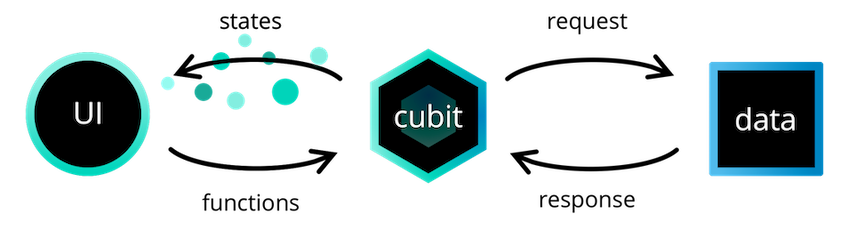
\includegraphics[width=1\textwidth]{img/cubit.png}
	\end{center}
	\caption{{\color{dgray}Model struktury wzorca projektowego BLoC.}} 
	\label{struktura_BLoC}
\end{figure}  

BLoC (Business Logic Component) - wzorzec projektowy pomagający oddzielić elementy wizualne projektu od części logiki działania programu. Dzieli projekt na trzy główne komponenty UI, cubit, data.

Warstwa UI jest odpowiedzialna za część wizualną aplikacji, cubit jest warstwą zawierającą mechanizmy działania aplikacji oraz pomostem pomiędzy interfejsem użytkownika, a zewnętrznymi danymi, natomiast warstwa data komunikuje się z zewnętrznymi instancjami (serwer, baza danych).\\

Cubit komunikuje się z warstwą danych poprzez funkcje asynchroniczne. Natomiast chcąc wpłynąć na zmianę wyglądu aplikacji korzysta z programowania reaktywnego. Mianowicie wysyła poszczególne stany strumieniem, którego dany element interfejsu aplikacji nasłuchuje. Stan jest to klasa reprezentująca dany stan poszczególnego elementu aplikacji. Relacja w drugą stronę polega na wywoływaniu bezpośrednio funkcji (synchronicznej lub asynchronicznej) na instancji cubita.

\section{Firebase}

Rolę serwera i bazy danych pełni platforma Firebase. Technologia ta, zarządzana również przez Google, określana jest jako Backend-as-a-Service. Firebase dostarcza wiele funkcjonalności
wspierające tworzenie projektów w tym między innymi uwierzytelnianie użytkowników, bazę danych NoSQL, hosting oraz API odpowiedzialne za komunikację. Usługi, które świadczy Firebase są bezpłatne, jeśli nie przekroczą pewnego z góry ustalonego limitu zdefiniowanego dla poszczególnej funkcjonalności. \\

\begin{figure}[h!]
	\begin{center}
		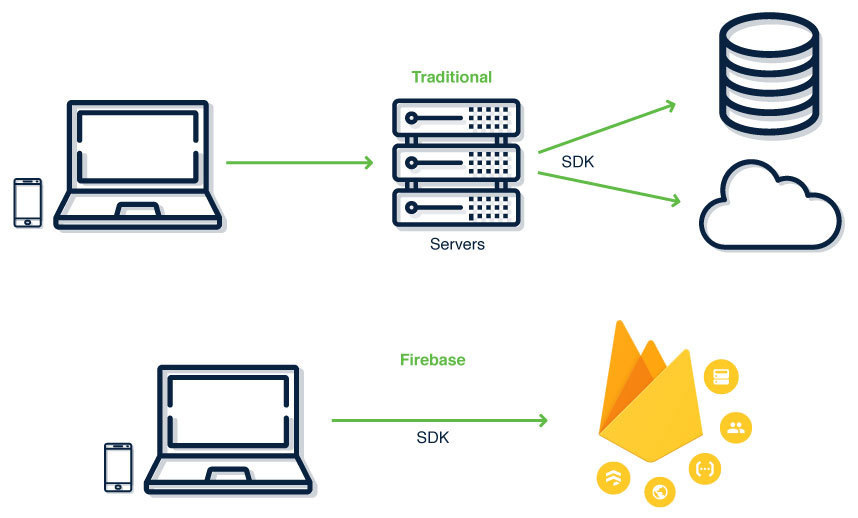
\includegraphics[width=0.7\textwidth]{img/firebase.png}
	\end{center}
	\caption{{\color{dgray} Porównanie struktury tradycyjnego serwera z platformą Firebase.}} 
	\label{struktura_firebase}
\end{figure}

\subsection{Firestore}

Firestore jest to baza danych NoSQL w chmurze. Jej strukturą są kolekcje, które zawierają dokumenty, które te z kolei zawierają dane, ale także mogą zawierać kolejne kolekcje. Definiując zapytanie do bazy danych zwracane są jedynie dokumenty z poszczególnej kolekcji lub grup kolekcji. Firestore umożliwia tworzenie prostych zapytań SQL, które filtruje wyniki na podstawie wartości danych znajdujących się w dokumencie. 

Firebase umożliwia po stronie klienta implementacje słuchaczy, którzy będą niezwłocznie informowani, gdy w obserwowanym dokumencie zaszła zmiana. 

Firestore umożliwia konfigurację dostępu do bazy danych za pomocą definiowania reguł bezpieczeństwa. Dla każdego dokumentu oraz pola można zdefiniować zakres dostępu (czytanie, modyfikacja, usuwanie) dla poszczególnego użytkownika.


\subsection{Funkcje Firebase}

Umożliwiają zaimplementowanie własnego kodu po stronie serwera. Są wywoływane poprzez zapytania HTTPS lub w odpowiedzi na zdarzenia powstałe w bazie danych Firestore. 
Możliwe jest wywoływanie bezpośrednio z poziomu aplikacji. Do zapytania dołączane są tokeny uwierzytelniania Firebase i tokeny sprawdzania aplikacji. Dostępne są dwa języki programowania, w których można zaimplementować funkcje Firebase. Można wybrać język Javascript lub jego odpowiednik ze statycznym typowaniem Typescript. \\

\subsection{Konsola Firebase}

Jest to strona internetowa, która oferuje dostęp do wszystkich funkcjonalności Firebase. Aby korzystać z platformy Firebase należy założyć tam własny projekt i skonfigurować go z docelową aplikacją. Po wstępnej konfiguracji otrzymuje się panel kontroli nad platformą Firebase dla projektu. Widzi się cały ruch generowany przez klientów w poszczególnych funkcjonalnościach np. liczba zapisów do bazy danych. Za pomocą konsoli można konfigurować i modyfikować każdą usługę. Zapewnia bezpośrednio dostęp do bazy danych, zarządzanie zarejestrowanymi użytkownikami, monitorowanie procesu działania serwisu. 

\subsection{Emulator}

Korzystając z funkcjonalności funkcji Firebase napotyka się na problem długiego czasu oczekiwania na zaktualizowanie kodu źródłowego programisty w chmurze Firebase (czas trwania około minuty). Oczekiwanie dłuższe niż parę sekund sprawia, że czas tworzenia kodu źródłowego po stronie serwera znacząco się wydłuża. Kolejną sprawą jest fakt, że w trakcie, gdy dany projekt jest już dostępny dla użytkowników, nie jest wskazana jego modyfikacja. Zatem trzeba tworzyć kopie projektu, które przeznaczone są do modyfikacji, co w przypadku, gdy nad projektem pracuje wielu programistów, staje się jeszcze bardziej nieefektywne. Ostatnim aspektem są koszty. W momencie programowania i testowania funkcjonalności serwera może dochodzić do generowania dużej ilości zapytań, co z kolei sumuje się do liczby zapytań i ewentualnych płatności. \\

Z powodu wyżej wymienionych problemów wraz z rozwojem platformy Firebase w 2019 roku oficjalnie został zaprezentowany Firebase Local Emulators. Emulator ten pozwala uruchomić wszystkie usługi Firebase lokalnie na własnym komputerze. Dzięki czemu szybko można nanieść zmiany w funkcjach Firebase, nie modyfikując właściwego projektu, a wykonywane zapytania nie są zliczane. \\

Każda usługa udostępniana przez platformę Firebase ma swój własny emulator, który jest uruchamiany na osobnym porcie. Zatem można uruchomić jedynie te emulatory tych funkcjonalności, które są wykorzystywane w projekcie. Ponadto fakt uruchomienia lokalnie funkcji Firebase  umożliwia debugowanie kodu.



